% This file should be compiled as such: PdfLatex -> Bibtex -> PdfLatex (x2)


\documentclass[10pt,a4paper]{article}



\usepackage[utf8]{inputenc}
\usepackage{amsmath}
\usepackage{amsfonts}
\usepackage{amssymb}
\usepackage{outlines}
\usepackage{xcolor}

\usepackage{lineno}
\renewcommand\linenumberfont{\normalfont\small\sffamily}
\linenumbers

\usepackage{graphicx}
\graphicspath{{../pics/}}

\usepackage{natbib}



\author{Jordan Wingenroth, Candace Yee, Justin Nghiem, and Laurel Larsen}



\title{Modeling effective collector efficiency of sparse and dense arrays of cylindrical collectors in varying states of flow velocity and turbulence}



\begin{document}



\maketitle



\paragraph{Editing notes:} 

\textcolor{red!75!green}{Parenthetical insertions in this color are author/editor notes referring to the preceding word or phrase}



\paragraph{Figures:}

I'm aiming for 10-12 figures; 3 methods, 7 results or thereabouts:

\begin{itemize}

\item Methods: Direct interception and capture efficiency diagram

\item Methods: Particle size distribution

\begin{figure}[h]
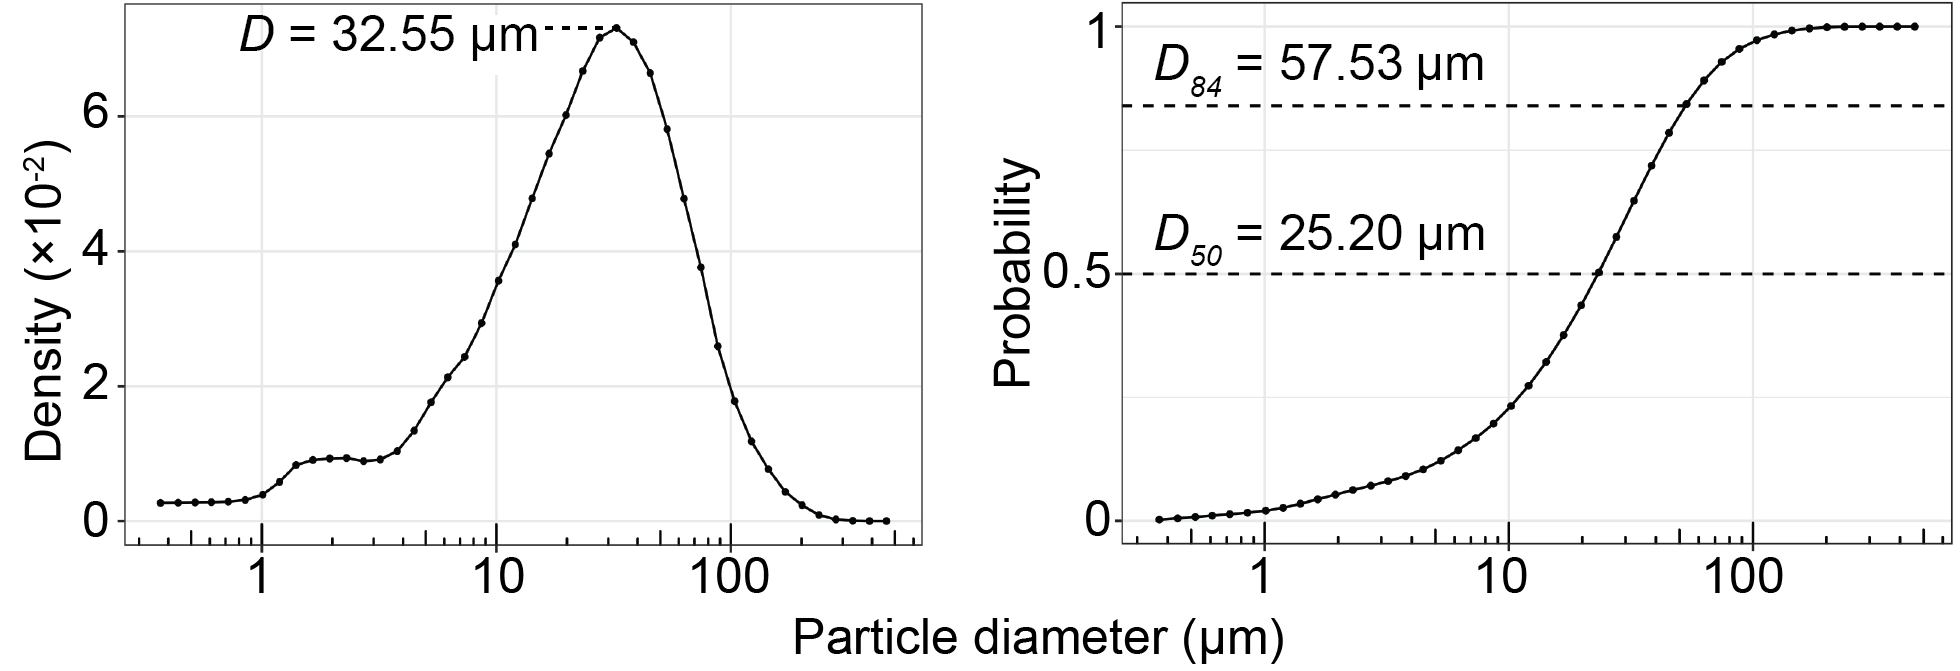
\includegraphics[width=10cm]{wf5-200sizedist.png}
\centering
\caption{Walnut shell particle size distribution}
\end{figure}

\item Methods: Flume floorplan

\end{itemize}



\section{Introduction}



\section{Methods}

\subsection{Theoretical Background}

Suspended particles in flowing water (i.e., waterborne particles) are subject to numerous physicochemical interactions \textcolor{red!75!green}{(better word?)}. Interactions stemming from fluid mechanics include grav



\subsection{Suspended Particle Concentration Model}
\marginpar{Note: Same subsection title as Fauria 2015. Should we change? Any ideas?}



\subsection{Experimental Methods}
\marginpar{Note: Same subsection title as Fauria 2015. Should we change? Any ideas?}



\subsubsection{Materials}



\subsubsection{Particle Concentration Run Protocols}



\subsubsection{Flow Characterization Run Protocols}



\subsection{Statistical Analysis}



\section{Results}

Example citation \citep{Fauria_2015}.



\section{Discussion}



\bibliographystyle{apalike}
\bibliography{refs}



\end{document}

